\chapter{Serie e trasformata di Fourier}

\section{Serie di Fourier esponenziale}
Dato un segnale periodico $s(t)$ di frequenza $f_0=\frac{1}{T}$ e periodo $T$ tale che $s(t)=s(t+k T)$, è possibile esprimerlo come somma di infinite sinusoidi pesate di frequenza multipla di $f_0$, $f_k=k f_0=\frac{k}{T}$.

\begin{definizione}
Dato il segnale periodico $s(t)=s(t+k T)$ si definisce la sua rappresentazione in \textsc{serie di Fourier} in forma di esponenziali complessi:
\begin{equation}\label{eq:serie_fourier}\index{serie!di Fourier}
s(t)=\sum_{k=-\infty}^{+\infty} c_k \e{\imath 2\pi k f_0 t}
\end{equation}
\end{definizione}
Le sinusoidi pesate sono espresse in forma di esponenziali complessi ricordando le formule di Eulero
\begin{equation}\e{\imath x}=\cos{x}+\imath\sen{x}\qquad\cos{x}=\frac{\e{\imath x}+\e{-\imath x}}{2}\qquad\sen{x}=\frac{\e{\imath x}-\e{-\imath x}}{2\imath}\end{equation}
I coefficienti $c_k$ costituiscono il peso o contributo della sinusoide a frequenza $f_k$ e si calcolano come
\begin{equation}\label{eq:serie_fourier_coef}\index{serie!di Fourier!coefficienti}
c_k=\frac{1}{T}\intd{-\frac{T}{2}}{\frac{T}{2}}{s(t)\e{-\imath 2\pi k f_0 t}}{t}
\end{equation}
Si può verificare sostituendo $s(t)$
\[c_k=\frac{1}{T}\intd{-\frac{T}{2}}{\frac{T}{2}}{ \left[\sum_{n=-\infty}^{+\infty} c_n \e{\imath 2\pi n f_0 t}\right] \e{-\imath 2\pi k f_0 t}}{t} = \frac{1}{T}\intd{-\frac{T}{2}}{\frac{T}{2}}{ \sum_{n=-\infty}^{+\infty} c_n \e{\imath 2\pi (n-k) f_0 t} }{t} \]
ipotizzando la convergenza della serie $s(t)$ ed essendo gli operatori $\sum$ e $\int$ lineari posso invertirne l'ordine
\[\begin{split}=&\frac{1}{T}\sum_{n=-\infty}^{+\infty} c_n \intd{-\frac{T}{2}}{\frac{T}{2}}{\e{\imath 2\pi(n-k)f_0 t}}{t}
=\frac{1}{T}\sum_{n=-\infty}^{+\infty} c_n \bound{-\frac{T}{2}}{\frac{T}{2}}{\frac{\e{\imath 2\pi(n-k)\frac{1}{T}t}}{\imath 2\pi(n-k)\frac{1}{T} }}\\
=&\frac{1}{T}\sum_{n=-\infty}^{+\infty} c_n T \frac{\e{\imath \pi(n-k)}-\e{-\imath\pi(n-k)}}{2\imath\pi(n-k)}
=\sum_{n=-\infty}^{+\infty} c_n \frac{\sen{\pi(n-k)}}{\pi(n-k)}
=\sum_{n=-\infty}^{+\infty} c_n \sinc{n-k} = c_k
\end{split}\]
essendo definito il $\sinc{x}=\frac{\sen{\pi x}}{\pi x}$, si ha che sinusoidi a frequenza diversa risultano ortogonali tra loro ovvero $\sinc{n-k}=\begin{cases}
1 & n=k \\ 0 & n\neq k\end{cases}$, l'integrale sul periodo del prodotto da contributo nullo e la sommatoria per $n$ si riduce al solo contributo per $n=k$.

I coefficienti $c_k$ sono numeri complessi $c_k=\abs{c_k}\e{\imath\theta_k}$ con ampiezza e fase associati alla armonica di frequenza $f_k$.

Il coefficiente $c_0$ corrispondente alla frequenza nulla si dice \textsc{componente continua} del segnale ed è pari al valor medio del segnale periodico in un periodo:
\begin{equation}c_0=\frac{1}{T}\intd{-\frac{T}{2}}{\frac{T}{2}}{s(t)}{t} \end{equation}

\begin{nota}Nei sistemi reali è sempre presente rumore per cui i termini $c_k$ ad un certo punto non danno contributi utili ad alte frequenze quindi posso sommare un numero finito di termini $c_0 + c_1\e{\imath 2\pi f_0 t}+c_{-1}\e{-\imath 2\pi f_0 t}+\dots\approx s(t)$.\end{nota}

\section{Condizioni di esistenza Dirichlet}\index{serie!di Fourier!condizioni Dirichlet}
Perché converga lo sviluppo in serie di Fourier del segnale $s(t)$ sono sufficienti le seguenti condizioni di esistenza:
\begin{enumerate}
\item $s(t)$ sia assolutamente integrabile in un periodo: $\intd{0}{T}{\abs{(s(t)}}{t}<+\infty$
\item $s(t)$ abbia nel periodo un numero finito di massimi e minimi
\item $s(t)$ abbia nel periodo un numero finito di discontinuità di I specie\footnote{Esistono finiti $\lim\limits_{t\to t_0+}s(t)\neq\lim\limits_{t\to t_0-}s(t)$, discontinuità I specie eliminabile $s(t_0)=\frac{s(t_0^+)-s(t_0^-)}{2}$}
\end{enumerate}
\begin{nota}Le condizioni sono molto restrittive ai fini pratici, anche segnali elementari come l'impulso e il gradino non ammettono sviluppo in serie di Fourier sotto tali condizioni.\end{nota}

\section{Serie di Fourier di sinusoidi}
Lo sviluppo in serie di Fourier può essere espresso come serie somma di seni e coseni o sinusoidi
\[\begin{split} s(t)&=\sum_{k=0}^{+\infty}\left[ a_k \sen{2\pi\frac{k}{T}t} + b_k \cos{2\pi\frac{k}{T}t}\right] \\
&=\sum_{k=0}^{+\infty}A_k\left[\sen{2\pi\frac{k}{T}t+\phi_k}\right] =\sum_{k=0}^{+\infty}A_k\left[\sen{2\pi\frac{k}{T}t}\Cos\phi_k +\cos{2\pi\frac{k}{T}t}\Sen\phi_k \right]
\end{split}\]
dove $a_k,b_k \in\R,\,\begin{cases}a_k=A_k\Cos\phi_k \\b_k=A_k\Sen\phi_k \end{cases}\implies\begin{cases}A_k^2=a_k^2+b_k^2\\ \tg\phi_k=\frac{b_k}{a_k} \end{cases}\implies\begin{cases}A_k=\sqrt{a_k^2+b_k^2}\\ \phi_k=\arctg\frac{b_k}{a_k} (+\pi\text{ se }a_k<0) \end{cases}$

I coefficienti $a_k$ e $b_k$ si calcolano come
\[a_k=\frac{2}{T}\intd{-\frac{T}{2}}{+\frac{T}{2}}{s(t)\sen{2\pi\frac{k}{T}t}}{t} \qquad b_k=\frac{2}{T}\intd{-\frac{T}{2}}{+\frac{T}{2}}{s(t)\cos{2\pi\frac{k}{T}t}}{t}\]
che per $k=0$ si semplificano nei coefficienti $a_0=0 \quad b_0=\frac{1}{T}\intd{0}{T}{s(t)}{t}$

\section{Equivalenza tra serie di Fourier}
Si dimostra che le serie di Fourier espresse come somma di esponenziali complessi e come somma di sinusoidi sono equivalenti.

\begin{proof}[Dim.]
\[s(t)=\sum_{k=-\infty}^{+\infty} c_k \e{\imath 2\pi\frac{k}{T}t} = \sum_{k=0}^{+\infty}\left[ a_k \sen{2\pi\frac{k}{T}t} + b_k \cos{2\pi\frac{k}{T}t}\right]
\]

Si vede che $\qquad b_0=c_0 \qquad b_k=c_k+c_{-k} \qquad a_k=\imath (c_k-c_{-k})$

Infatti si può scrivere
\[\begin{split}\sum_{k=-\infty}^{+\infty} & c_k \e{\imath 2\pi\frac{k}{T}t} = c_0+ \sum_{k=1}^{+\infty} \left[ c_k \e{\imath 2\pi\frac{k}{T}t} + c_{-k} \e{-\imath 2\pi\frac{k}{T}t} \right] = \\
&= c_0 + \sum_{k=1}^{+\infty} {\left\lbrace c_k \left[\cos{2\pi\frac{k}{T}t}+\imath\sen{2\pi\frac{k}{T}t}\right]
+c_{-k}\left[\cos{2\pi\frac{k}{T}t}-\imath\sen{2\pi\frac{k}{T}t}\right] \right\rbrace}=\\
&= c_0 + \sum_{k=1}^{+\infty} {\left[(c_k+c_{-k}) \cos{2\pi\frac{k}{T}t}+
(c_k-c_{-k})\imath\sen{2\pi\frac{k}{T}t}\right] }\end{split}\]
\end{proof}

\[b_k=c_k+c_{-k}=\frac{1}{T}\intd{-\frac{T}{2}}{\frac{T}{2}}{s(t)\left[\e{\imath 2\pi\frac{k}{T}t}+\e{-\imath 2\pi\frac{k}{T}t}\right]}{t}=\frac{2}{T}\intd{-\frac{T}{2}}{\frac{T}{2}}{s(t)\cos{2\pi\frac{k}{T}t}}{t} \]
\[a_k=\imath(c_k-c_{-k})=\imath\frac{1}{T}\intd{-\frac{T}{2}}{\frac{T}{2}}{s(t)\left[\e{\imath 2\pi\frac{k}{T}t}-\e{-\imath 2\pi\frac{k}{T}t}\right]}{t}=\frac{2}{T}\intd{-\frac{T}{2}}{\frac{T}{2}}{s(t)\sen{2\pi\frac{k}{T}t}}{t} \]

\begin{nota}L'informazione del segnale è contenuta nei pesi $c_k$ o equivalentemente $a_k$ e $b_k$.
\end{nota}

\section{Simmetrie coefficienti}
Per un segnale reale $s(t)\in\R$ la parte immaginaria deve essere nulla ovvero i termini $c_k=\Re c_k + \imath \Im c_k$ devono essere tali che $c_k \e{\imath 2\pi\frac{k}{T}t}+ c_{-k}\e{-\imath 2\pi\frac{k}{T}t}\in\R,\forall k$
\[c_k+c_{-k}\in\R \implies \Im c_k+\Im c_{-k}=0 \implies \Im c_k=-\Im c_{-k}\]
\[c_k-c_{-k} \text{ immaginario puro } \implies \Re c_k -\Re c_{-k}=0 \implies \Re c_k=\Re c_{-k} \]

Per un segnale reale quindi i coefficienti sono complessi e coniugati $c_k=\conj{c_{-k}}$ (\textsc{simmetria Hermitiana})

Per un segnale reale e pari si ha $a_k=0\,\forall k \implies c_k=c_{-k}$

Per un segnale reale e dispari si ha $b_k=0\,\forall k \implies c_k=-c_{-k}$

\section{Esempio serie di Fourier di un'onda quadra}
\begin{esempio}
Segnale onda quadra di periodo T durata $\tau$ in fig.\ref*{fig:onda_quadra} \[s(t)=\sum_{n=-\infty}^{+\infty}\rect{\frac{t-n T}{\tau}}\]

\begin{figure}[ht]
\begin{center}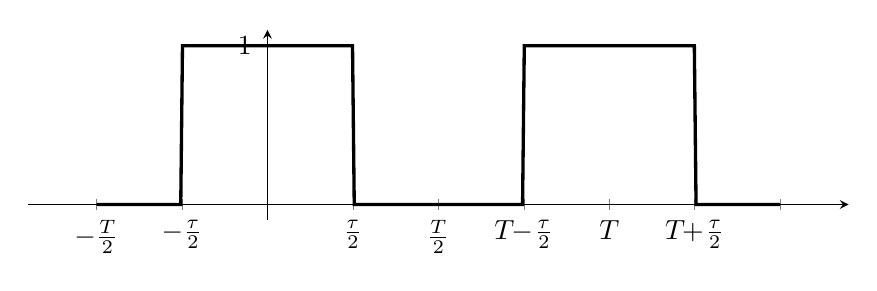
\begin{tikzpicture}
	\begin{axis}[width=12cm, height=4cm, axis lines=middle,no markers,enlargelimits,xtick={-1,-.5,0,.5,1,1.5,2,2.5,3},xticklabels={$-\frac{T}{2}$,$-\frac{\tau}{2}$,$0$,$\frac{\tau}{2}$,$\frac{T}{2}$,$T\!\!-\!\frac{\tau}{2}$,$T$,$T\!\!+\!\frac{\tau}{2}$},ytick={0,1}]
	\addplot [very thick,samples=200,domain=-1:1]  {abs(x)<.5?1:0};
	\addplot [very thick,samples=200,domain=1:3]  {abs(x-2)<.5?1:0};
	\end{axis}
	\end{tikzpicture}
\end{center}
\caption{Onda quadra}\label{fig:onda_quadra}
\end{figure}
Il segnale è reale pari ($c_k=c_{-k}$), i coefficienti della serie di Fourier si calcolano applicando la formula \ref{eq:serie_fourier_coef}:
\[\begin{split}c_k&=\frac{1}{T}\intd{-\frac{T}{2}}{\frac{T}{2}}{s(t)\e{-\imath 2\pi\frac{k}{T}t}}{t}
=\frac{1}{T}\intd{-\frac{\tau}{2}}{\frac{\tau}{2}}{\e{-\imath 2\pi\frac{k}{T}t}}{t}
=\frac{1}{T}\bound{-\frac{\tau}{2}}{\frac{\tau}{2}}{ \frac{\e{-\imath 2\pi\frac{k}{T}t}}{-\imath 2\pi\frac{k}{T}}}=\\
&=\frac{1}{\pi k} \frac{-\e{-\imath 2\pi\frac{k}{T}\frac{\tau}{2}}+\e{\imath 2\pi\frac{k}{T}\frac{\tau}{2}}}{\imath 2}
=\frac{\sen{\pi \tau \frac{k}{T}}}{\pi k}
=\frac{\tau}{T}\frac{\sen{\pi k \frac{\tau}{T}}}{\pi k \frac{\tau}{T}}
=\frac{\tau}{T}\sinc{k \frac{\tau}{T}}
\end{split}\]

\begin{figure}[h!]
\centering
{\begin{tikzpicture}[scale=.6]
	\begin{axis}[width=10cm,axis lines=middle,no markers,enlargelimits,xscale=1.5,xtick={-3,-1,0,1,3},xticklabels={$-T$,$-\tau$,0,$\tau$,$T$},ytick={0,1},yticklabels={0,$\frac{\tau}{T}$}]
	\addplot [dashed,domain=-7:7,samples=100] {sin(pi*x/3)/(pi*x/3)};
	\addplot+[only marks,samples at={-3,-2,-1,0.001,1,2,3}]
	{sin(pi*x/3)/(pi*x/3)};
	\end{axis}\end{tikzpicture}}
\caption{Valori coefficienti $c_k=\frac{\tau}{T}\sinc{\frac{t}{T}}$}
\label{fig:sinc_onda_quadra}
\end{figure}
\end{esempio}

\section{Proprietà della serie di Fourier}
\subsection{Linearità}L'integrale è un operatore lineare pertanto una combinazione lineare di segnali trasforma linearmente i coefficienti della serie
\[ y(t)=a s_1(t)+ b s_2(t)\]
\[ c_{y k}= a c_{1 k} + b c_{2 k} \]

\subsection{Traslazione nel tempo}
Un segnale traslato nel tempo $s(t-\tau)$, ritardato o anticipato di un tempo $\tau$, vede i coefficienti modificati nella fase $c_r^{'}=c_k \e{-\imath 2\pi\frac{k}{T}\tau}$

\begin{proof}[Dim.]
\[ \intd{-\frac{T}{2}}{\frac{T}{2}}{s(t-\tau)\e{-\imath 2\pi\frac{k}{T}t}}{t} \]
effettuando il cambio di variabile $t-\tau=x$, $t=x+\tau$, $\diff t=\diff x$
\[\intd{-\frac{T}{2}}{\frac{T}{2}}{s(x)\e{-\imath 2\pi\frac{k}{T}x}\e{-\imath 2\pi\frac{k}{T}\tau}}{x} =
\e{-\imath 2\pi\frac{k}{T}\tau} \intd{-\frac{T}{2}}{\frac{T}{2}}{s(x)\e{-\imath 2\pi\frac{k}{T}x}}{x}\]
si nota anche che data la periodicità per $\tilde{\tau}=\tau+N T$
\[\e{-\imath 2\pi\frac{k}{T}\tilde{\tau}}=
\e{-\imath 2\pi\frac{k}{T}\tau} \underbrace{\e{-\imath 2\pi\frac{k}{T}N T}}_{1}=\e{-\imath 2\pi\frac{k}{T}\tau}
\]
\end{proof}

\section{Potenza segnale periodico (Teo. Parseval)}
La potenza del segnale periodico è contenuta nei suoi toni armonici:
\begin{equation}\label{eq:teo_Parseval}\index{Teorema!Parseval}
P=\sum_{k=-\infty}^{+\infty}{\abs{c_k}^2}
\end{equation}

\begin{proof}[Dim.]
\[\begin{split}P&= \frac{1}{T}\intd{-\frac{T}{2}}{\frac{T}{2}}{\abs{s(t)}^2}{t}=\frac{1}{T}\intd{-\frac{T}{2}}{\frac{T}{2}}{ \left(\sum_{k=-\infty}^{+\infty}{c_k\e{\imath 2\pi\frac{k}{T}t}}\right) \left(\sum_{n=-\infty}^{+\infty}{c_n\e{\imath 2\pi\frac{n}{T}t}}\right)}{t}= \\
&=\frac{1}{T}\intd{-\frac{T}{2}}{\frac{T}{2}}{ \left(\sum_{k=-\infty}^{+\infty}{c_k\e{\imath 2\pi\frac{k}{T}t}}\right) \left(\sum_{n=-\infty}^{+\infty}{\conj{c_n}\e{-\imath 2\pi\frac{n}{T}t}}\right)}{t}= \\
\intertext{il prodotto di armoniche ortogonali da contributo non nullo solo per $n=k$, pertanto}
&=\frac{1}{T}\intd{-\frac{T}{2}}{\frac{T}{2}}{ \left(\sum_{k=-\infty}^{+\infty}{c_k \conj{c_k} \e{\imath 2\pi\frac{k}{T}t} \e{-\imath 2\pi\frac{k}{T}t}}\right)}{t}= \\
&=\frac{1}{T}\intd{-\frac{T}{2}}{\frac{T}{2}}{\sum_{k=-\infty}^{+\infty}{\abs{c_k}^2}}{t}=
\frac{1}{T}\sum_{k=-\infty}^{+\infty}{\abs{c_k}^2}\intd{-\frac{T}{2}}{\frac{T}{2}}{}{t}=\sum_{k=-\infty}^{+\infty}{\abs{c_k}^2}
\end{split}\]
\end{proof}

\section{Trasformata di Fourier}
Per segnali non periodici la potenza del segnale non è concentrata nei moti armonici ma è distribuita con continuità a tutte le frequenze dello spettro.

Il segnale aperiodico è rappresentabile come l'\textsc{integrale di Fourier}
\begin{equation}
s(t)=\intinf{S(f)\e{\imath 2\pi f t}}{f}
\end{equation}

La funzione complessa $S(f)$, nella variabile continua $f$, rappresenta la \textsc{trasformata di Fourie}r del segnale $s(t)$
\begin{equation}
S(f)=\intinf{s(t)\e{-\imath 2\pi f t}}{t}
\end{equation}
Il modulo e la fase della grandezza complessa definiscono
\[\abs{S(f)} \text{ spettro di ampiezza} \quad \angle S(f) \text{ spettro di fase}\]

\subsection{Condizioni di esistenza di Dirichlet}
I criteri di Dirichlet condizioni sufficienti per l'esistenza della trasformata di Fourier di un segnale $s(t)$:
\begin{enumerate}
\item $\intinf{\abs{s(t)}}{t}<\infty$ (assolutamente integrabile)
\item numero finito di discontinuità (tutte di I specie)
\item numero finito di max e min
\end{enumerate}
\begin{nota}Le condizioni non sono necessarie: alcune funzioni pur non soddisfacendo le tre condizioni sono trasformabili.\end{nota}
\begin{esempio}
Il segnale aperiodico di durata limitata $\tau$ ha trasformata di Fourier
\[s(t)=\rect{\frac{t}{\tau}}\quad\fourier{\rect{\frac{t}{\tau}}}=\tau\sinc{f\tau} \]

\begin{figure}[h!]
\centering
\subfloat[][$s(t)=\rect{\frac{t}{\tau}}$]
{\begin{tikzpicture}[scale=.6]
	\begin{axis}[axis lines=middle,no markers,enlargelimits,xscale=1.5,xtick={-.5,0,.5},xticklabels={$-\frac{\tau}{2}$,$0$,$\frac{\tau}{2}$},ytick={0,1}]
	\addplot [very thick,samples=200,domain=-1:1]  {abs(x)<.5?1:0};
	\end{axis}
\end{tikzpicture}}\qquad
\subfloat[][$S(f)=\tau\sinc{f\tau}$]
{\begin{tikzpicture}[scale=.6]
	\begin{axis}[axis lines=middle,no markers,enlargelimits,xscale=1.5,xtick={-9.424,-6.283,-3.141,0,3.141,6.283,9.424},ytick={0,1},xticklabels={$-3\tau$,$-2\tau$,$-\tau$,$0$,$\tau$,$2\tau$,$3\tau$},yticklabels={$0$,$\tau$}]
	\addplot [very thick,domain=-3.5*pi:3.5*pi,samples=100] {sin(x)/x};
	\end{axis}\end{tikzpicture}}
\end{figure}

\[\begin{split}S(f)&=\intinf{s(t)\e{-\imath 2\pi f t}}{t}
=\intd{-\frac{\tau}{2}}{\frac{\tau}{2}}{1\cdot\e{-\imath 2\pi f t}}{t}
=\bound{-\frac{\tau}{2}}{\frac{\tau}{2}}{\frac{\e{-\imath 2\pi f t}}{-\imath 2\pi f}}=\\
&=\frac{-\e{-\imath 2\pi f\frac{\tau}{2}}+\e{\imath 2\pi f\frac{\tau}{2}}}{\imath 2\pi f}
=\tau\frac{\sen{\pi f\tau}}{\pi f\tau}
=\tau\sinc{f\tau}
\end{split}\]
\end{esempio}

\section{Proprietà trasformata di Fourier}
\subsection{Simmetria}
La trasformata di un segnale reale $s(t)$ gode di simmetria hermitiana $\conj{S}(f)=S(-f)$
\begin{equation}\conj{S}(f)=\intinf{s(t)\e{+\imath 2\pi f t}}{t}=S(-f)\end{equation}
Espresso nella parte reale e immaginaria
\[S(f)=S_R(f)+\imath S_I(f)=\intinf{s(t)\cos{2\pi f t}}{t}-\imath\intinf{s(t)\sen{2\pi f t}}{t}\]
Se $s(t)$ è reale pari, la trasformata è reale pari: \[\conj{S}(f)=\conj{[S_R(f)]}=S(-f)\] \[S_R(f)=S_R(-f)\]
Se $s(t)$ è reale dispari, la trasformata è immaginaria pura dispari:
\[\conj{S}(f)=\conj{[+\imath S_I(f)]}=-\imath S_I(f)=\imath S_I(-f)\] \[S_I(f)=-S_I(-f)\]

\subsection{Linearità}
La trasformata di Fourier di combinazione lineare di segnali gode di linearità
\begin{equation}
\fourier{a x(t)+ b y(t)}= a X(f)+ b Y(f)
\end{equation}

\begin{proof}[Dim.]
Applicando la definizione di trasformata e per la linearità dell'operatore integrale
\[ \intinf{\left[a x(t)+ b y(t)\right]\e{-\imath 2\pi f t}}{t}= a\intinf{x(t)\e{-\imath 2\pi f t}}{t} + b\intinf{y(t)\e{-\imath 2\pi f t}}{t}= a X(f) + b Y(f) \]
\end{proof}

\subsection{Traslazione nel tempo}
La trasformata di Fourier di un segnale anticipato o ritardato nel tempo modifica lo spettro di fase del segnale
\begin{equation}
\fourier{s(t-\tau)}= S(f)\e{-\imath 2\pi f \tau}
\label{eq:trasf_Fourier_trasl}
\end{equation}
\begin{proof}[Dim.]
Applicando un cambio di variabile $\alpha=t-\tau$ e la definizione di trasformata
\[\intinf{s(t-\tau)\e{-\imath 2\pi f t}}{t}=
\intinf{s(\alpha)\e{-\imath 2\pi f\alpha}\e{-\imath 2\pi f\tau}}{\alpha}=S(f)\e{-\imath 2\pi f\tau}\]
\end{proof}

\subsection{Ribaltamento}
La trasformata di Fourier di un segnale invertito nel tempo ha lo spettro del segnale ribaltato nelle frequenze
\begin{equation}\fourier{s(-t)}=S(-f)\end{equation}
\begin{proof}[Dim.]
Applicando un cambio di variabile $\alpha=-t$ e la definizione di trasformata
\[\intinf{s(-t)\e{-\imath 2\pi f t}}{t}=
\intinf{s(\alpha)\e{-\imath 2\pi (-f)\alpha}}{\alpha}=S(-f)\]
\end{proof}

\subsection{Cambiamento di scala temporale}
La trasformata di Fourier di un segnale compresso o dilatato nella scala dei tempi dilata o comprime lo spettro delle frequenze del segnale
\begin{equation}\label{eq:trasf_Fourier_scala}
\fourier{s(a t)}=\frac{1}{\abs{a}}\,\f{S}{\frac{f}{a}}
\end{equation}
\begin{proof}[Dim.] Applicando un cambio di variabile $\alpha=a t, t=\frac{\alpha}{a}, \diff t=\frac{\diff\alpha}{a}$ e la definizione di trasformata
\[\intinf{s(a t)\e{-\imath 2\pi f t}}{t}=
\int_{-\infty}^{\infty}{s(\alpha)\e{-\imath 2\pi\frac{f}{a}\alpha}}{\frac{\diff\alpha}{\abs{a}}}=\frac{1}{\abs{a}}\,\f{S}{\frac{f}{a}}\]
\end{proof}

\subsection{Derivazione}
La trasformata di Fourier della derivata di un segnale
\begin{equation}
\fourier{s'(t)}=\imath 2\pi f\,S(f)
\end{equation}
\begin{proof}[Dim.] Si ha infatti che per un segnale derivabile $s(t)$
\[s(t)=\intinf{S(f)\e{\imath 2\pi f t}}{f}\implies s'(t)=\deriv{}{t}\intinf{S(f)\e{\imath 2\pi f t}}{f}=
\intinf{ \underbrace{\imath 2\pi f S(f)}_{\fourier{s'(t)}}\e{\imath 2\pi f t}}{f} \]
\end{proof}

\begin{nota}L'operatore derivata temporale di un segnale si comporta come un filtro passa alto perché nelle frequenze si ha il prodotto con il fattore $\imath 2\pi f$ che essendo proporzionale alla frequenza $f$ esalta in modulo le alte frequenze, mentre attenua le frequenze per $f\to 0$. La fase viene modificata di $\pm\frac{\pi}{2}$ a seconda del segno di $f$.\end{nota}

\subsection{Convoluzione nel tempo}
La trasformata di Fourier del prodotto di convoluzione di due segnali
\begin{equation}
\fourier{x(t)\ast y(t)}=X(f)\cdot H(f)
\label{eq:trasf_Fourier_conv}
\end{equation}
\begin{proof}[Dim.] Applicando la trasformata di Fourier al prodotto di convoluzione e l'eq.\ref{eq:trasf_Fourier_trasl}
\[\begin{split}& \intinf{ \left[\intinf{x(\tau)h(t-\tau)}{\tau}\right] \e{-\imath 2\pi f t}}{t} =
\intinf{ x(\tau) \left[\intinf{h(t-\tau)\e{-\imath 2\pi f t}}{t}\right]}{\tau}=\\
=& \intinf{ x(\tau) H(f)\e{-\imath 2\pi f \tau}}{\tau} = X(f) H(f) \end{split}\]
\end{proof}

\subsection{Dualità}
Nota la trasformata di Fourier $S(f)$ di un segnale $s(t)$ si ha che la trasformata di Fourier del segnale temporale $S(t)$ è per dualità $s(-f)$
\begin{equation}
\begin{split}
s(t) &\overset{\Fourier}{\to} S(f) \\
S(t) &\overset{\Fourier}{\to} s(-f)
\end{split}
\end{equation}
\begin{proof}[Dim.]
Nella tra il segnale e la sua trasformata $s(t)=\intinf{S(f)\e{+\imath 2\pi f t}}{f}$
si ha scambiando formalmente le variabili $t$ e $f$ \[s(f)=\intinf{S(t)\e{+\imath 2\pi f t}}{t}\]
cambiando variabile $f$ con $-f$
\[\fourier{S(t)}=\intinf{S(t)\e{-\imath 2\pi f t}}{t}=s(-f)\]
\end{proof}

\begin{esempio}
\begin{equation}
\begin{split}
\rect{t} &\overset{\Fourier}{\to} \sinc{f}\\
\sinc{t} &\overset{\Fourier}{\to} \rect{-f}=\rect{f}
\end{split}
\end{equation}
La proprietà di dualità consente di ottenere velocemente risultati che richiederebbero molti calcoli applicando la definizione.
\end{esempio}

\begin{esempio}\label{es:trasf_Fourier_conv}

\begin{figure}[h!]
\centering
\subfloat[][$s(t)=\rect{\frac{t}{T}}\ast\rect{\frac{t}{T}}$]
{\begin{tikzpicture}[scale=.67]
\begin{axis}[axis lines=middle,no markers,enlargelimits,xscale=1.2,xtick={-1,0,1},ytick={0,1},xticklabels={$-T$,0,$T$},yticklabels={0,$T$}]
\addplot [very thick]coordinates {(-2,0)(-1,0)(0,1)(1,0)(2,0)};
\end{axis}\end{tikzpicture}}\qquad
\subfloat[][$S(f)=T^2\Sinc^2(f T)$] {
\begin{tikzpicture}[scale=.7]
\begin{axis}[axis lines=middle,no markers,enlargelimits,xscale=1.5,xtick={-9.424,-6.283,-3.141,0,3.141,6.283,9.424},ytick={0,1},xticklabels={$-\frac{3}{T}$,$-\frac{2}{T}$,$-\frac{1}{T}$,$0$,$\frac{1}{T}$,$\frac{2}{T}$,$\frac{3}{T}$},yticklabels={$0$,$T^2$}]
\addplot [very thick,domain=-3.5*pi:3.5*pi,samples=100] { (sin(x)/x)^2 };
\end{axis}\end{tikzpicture}
}
\caption{Esempio \ref{es:trasf_Fourier_conv} convoluzione segnali rettangolari e trasformata}
\end{figure}

\[s(t)=\rect{\frac{t}{T}}\ast\rect{\frac{t}{T}}\]
Per la prop. di scala $\rect{\frac{t}{T}}\overset{\Fourier}{\to}T\sinc{f T}$ e per la prop. di convoluzione si ha
\[S(f)=T^2\Sinc^2(f T)\]
\end{esempio}

\subsection{Traslazione in frequenza}
L'anti-trasformata di Fourier del segnale traslato in frequenza $S(f-f_0)\overset{\Fourier^{-1}}{\rightarrow}s(t)\e{\imath 2\pi f_0 t}$

\begin{proof}[Dim.]
Applicando l'anti trasformata di Fourier allo spettro traslato in frequenza, con opportuno cambio di variabile $\alpha=f-f_0, f=f_0+\alpha, \diff\alpha=\diff f$
\[\intinf{S(f-f_0)\e{\imath 2\pi f t}}{f}=
\intinf{S(\alpha)\e{\imath 2\pi\alpha t}\e{\imath 2\pi f_0 t}}{\alpha}=\e{\imath 2\pi f_0 t} s(t) \]
\end{proof}

\subsection{Prodotto nel tempo $\to$ convoluzione in frequenza}
Dati due segnali $x(t)$ e $y(t)$ con le loro trasformate di Fourier $X(f)$ e $Y(f)$. La trasformata del segnale prodotto
\begin{equation}
\begin{split}
z(t) = x(t) y(t) &\overset{\Fourier}{\rightarrow} Z(f) = X(f)\ast Y(f)
\end{split}
\end{equation}

\begin{proof}[Dim.] Applicando la definizione
\[\begin{split}Z(f)&=\intd{t=-\infty}{+\infty}{z(t)\e{-\imath 2\pi f t}}{t}=\intd{t=-\infty}{+\infty}{x(t)y(t)\e{-\imath 2\pi f t}}{t}=\\
\intertext{sostituendo a $x(t)$ la sua espressione come integrale di Fourier}
&=\intd{t=-\infty}{+\infty}{\left[\intd{\nu=-\infty}{+\infty}{X(\nu)\e{\imath 2\pi\nu t}}{\nu}\right]y(t)\e{-\imath 2\pi f t}}{t}=\\
\intertext{invertendo l'ordine di integrazione}
&=\intd{\nu=-\infty}{+\infty}{X(\nu)\left[\intd{t=-\infty}{+\infty}{y(t)\e{-\imath 2\pi(f-\nu)t}}{t}\right]}{\nu}=\\
\intertext{si ha nella parentesi quadra la trasformata di $y(t)$ calcolata alla frequenza $f-\nu$}
&=\intd{\nu=-\infty}{+\infty}{X(\nu)Y(f-\nu)}{\nu} = X(f)\ast Y(f)
\end{split}\]
\end{proof}

\begin{nota}
Dato un segnale generico è possibile estrarre una finestra di durata limitata moltiplicando il segnale per un $\Rect$. Per la proprietà della trasformata del prodotto risulta che un segnale di durata limitata ha sempre banda a tutte le frequenze perché il $\Rect$ ha spettro infinito.
\end{nota}

\subsection{Teorema di Parseval}
Per i segnali di energia finita si può sempre calcolare la trasformata di Fourier. Per il teorema di Parseval
\begin{equation}E_s=\intinf{\abs{s(t)}^2}{t}=\intinf{\abs{S(f)}^2}{f}\label{eq:parseval}\end{equation}
che da indicazioni su come è distribuita l'energia del segnale alle varie frequenze. Per l'integrale di Fourier $s(t)=\intinf{S(f)\e{\imath 2\pi f t}}{t}$ il segnale $s(t)$ è la somma di infinite sinusoidi pesate da $S(f)$: che è anche l'integrale dei contributi infinitesimi di energia alle varie frequenze dello spettro.
\begin{nota}\`{E} importante notare che per la trasformata di Fourier cambiare l'energia ad una frequenza $f_0$ non comporta cambiamenti ad altre frequenze.\end{nota}
\begin{proof}[Dim.]
\[\begin{split}\intinf{\abs{s(t)}^2}{t}&=\intinf{s(t)\conj{s}(t)}{t}
=\intinf{s(t)\conj{\left[\intinf{S(f)\e{\imath 2\pi f t}}{f}\right]}}{t}=\\
&=\intinf{s(t)\intinf{\conj{S}(f)\e{-\imath 2\pi f t}}{f}}{t}=\intinf{\conj{S}(f)\intinf{s(t)\e{-\imath 2\pi f t}}{t}}{f}=\\
&=\intinf{\conj{S}(f)S(f)}{f}=\intinf{\abs{S(f)}^2}{f}\end{split}\]
\end{proof}

\begin{nota}Tutte le proprietà della trasformata di Fourier valgono sotto le condizioni di Dirichlet. Tali condizioni sono molto stringenti ai fini pratici, anche segnali elementari come l'impulso e il gradino non ammettono trasformata di Fourier. Le condizioni saranno superate con la trasformata generalizzata.\end{nota}

\subsection{Trasformata funzione generalizzata $\delta(t)$}
Per calcolare la trasformata di Fourier della funzione generalizzata delta di Dirac $\delta(t)$ si applica la definizione tenendo conto della proprietà campionatrice della $\delta(t)$
\begin{equation}
\fourier{\delta(t)}=\intinf{\delta(t)\e{-\imath 2\pi f t}}{t}=\restrict{\e{-\imath 2\pi f t}}{t=0}=1
\end{equation}
Da questo risultato per la funzione generalizzata e per il teorema di dualità è possibile calcolare la trasformata di Fourier del segnale ad energia infinita come il segnale costante
\begin{equation}
\fourier{1}=\delta(-f)=\delta(f)
\end{equation}
\[\fourier{c}=c\,\delta(f)\]

\subsection{Trasformata funzione generalizzata $\step(t)$}
La trasformata di Fourier della funzione gradino unitario ideale $\step(t)$ non esiste. Bisogna far ricorso alla trasformata con le funzioni generalizzate, definendo il gradino come
\[\step(t)=\frac{1}{2}+\frac{1}{2}\sgn(t)\]
\begin{equation}
\fourier{\step(t)}=\frac{1}{2}\delta(f)+\frac{1}{\imath 2\pi f}
\end{equation}
\begin{figure}[h!]\centering
\begin{tikzpicture}[scale=.6]
\begin{axis}[axis lines=middle,no markers,enlargelimits,xscale=1.5,xtick={-1,0,1},ytick={0,.5,1},yticklabels={$0$,$\frac{1}{2}$,$1$}]
\addplot [very thick]coordinates {(-1,0)(0,0)};
\addplot [only marks, samples at={0}]coordinates {(0,.5)};
\addplot [very thick]coordinates {(0,1)(1,1)};
\end{axis}\end{tikzpicture}
\caption{Funzione $\sgn(t)$}
\end{figure}

\begin{proof}[Dim.]
La trasformata della funzione $\sgn(t)$ si ottiene per dualità della trasformata della funzione $\frac{1}{t}\overset{\Fourier}{\to}-\imath\pi\sgn(f)$
\[\begin{split}&\fourier{\frac{1}{t}}=\intinf{\frac{1}{t}\e{-\imath 2\pi f t}}{t}= \underbrace{\intinf{\frac{1}{t}\cos{2\pi f t}}{t}}_{\stackrel{=0}{1/t \text{ dispari}}} -\imath\intinf{\frac{1}{t}=\sen{2\pi f t}}{t}=\\
&=-\imath 2\pi f\intinf{\frac{\sen{2\pi f t}}{2\pi f t}}{t}=-\imath 2\pi f\intinf{\sinc{2 f t}}{t}= -\imath\frac{2\pi f}{2\abs{f}} = -\imath\pi\sgn(f)
\end{split} \]
L'integrale nel tempo da $-\infty$ a $+\infty$ di un segnale è pari alla trasformata del segnale calcolata per $f=0$. La trasformata del $\sinc{t}\overset{\Fourier}{\to}\rect{f}$ per la prop. di dualità, la trasformata di $\sinc{2\alpha t}\overset{\Fourier}{\to}\frac{1}{2\abs{\alpha}}\rect{\frac{f}{2\alpha}}$ per la prop. di scala, calcolata per $f=0$ il $\rect{0}=1$, da cui
$\intinf{\sinc{2 f t}}{t}=\frac{1}{2\abs{f}}$.

Da $s(t)=\frac{1}{t}\overset{\Fourier}{\to} -\imath\pi\sgn(f)$, per dualità $S(t)\overset{\Fourier}{\to} s(-f)$ da cui \[\fourier{\sgn(t)}=\frac{1}{-\imath\pi}\frac{1}{-f}=\frac{1}{\imath\pi f}\] da cui il risultato per la trasformata generalizzata del gradino \[\fourier{\step(t)}]=\fourier{\frac{1}{2}+\frac{1}{2}\sgn(t)}=\frac{1}{2}\delta(f)+\frac{1}{\imath 2\pi f}\]
\end{proof}

\subsection{Teorema integrazione completo}\index{Teorema!integrazione completo}
Per un segnale definito come integrale di convoluzione con un gradino
\[y(t)=\intd{-\infty}{t}{x(\tau)}{\tau}=\intinf{x(\tau)\step(t-\tau)}{\tau}=x(t)\ast\step(t)\]
si può determinare la trasformata generalizzata
\begin{equation}
Y(f)=X(f) U(f)=\frac{1}{2} X(0) \delta(f) + \frac{X(f)}{\imath 2\pi f}
\end{equation}
che tiene conto nel primo termine della componente continua del segnale.

\subsection{Trasformate funzioni seno e coseno}
Dalla funzione generalizzata $\delta(t)\overset{\Fourier}{\rightarrow}1$ si hanno per il teo. traslazione del tempo e per il teo. dualità le trasformate di Fourier delle funzioni seno e coseno
\[\begin{split}\delta(t-t_0)&\overset{\Fourier}{\to}\e{-\imath 2\pi f t_0}\\
\e{\imath 2\pi f_0 t}&\overset{\Fourier}{\to}\delta(f-f_0)\end{split}\]
\begin{equation}
\cos{2\pi f_0 t}=\frac{\e{\imath 2\pi f_0 t}+\e{-\imath 2\pi f_0 t}}{2}\overset{\Fourier}{\to}\frac{\delta(f-f_0)+\delta(f+f_0)}{2}\end{equation}
\begin{equation}\sen{2\pi f_0 t}=\frac{\e{\imath 2\pi f_0 t}-\e{-\imath 2\pi f_0 t}}{2\imath}\overset{\Fourier}{\to}\frac{\delta(f-f_0)-\delta(f+f_0)}{2\imath}\end{equation}

\subsection{Modulazione}
Per il teorema trasformata del prodotto e la proprietà campionatrice della funzione generalizzata $\delta$ si ha il risultato notevole per cui la trasformata di un segnale modulato risulta
\begin{equation}\label{eq:fourier_modulazione_coseno}
s(t) \cos{2\pi f_0 t}\overset{\Fourier}{\to}\frac{1}{2}\left[S(f-f_0)+S(f+f_0)\right]
\end{equation}
\begin{equation}
s(t) \sen{2\pi f_0 t}\overset{\Fourier}{\to}\frac{1}{2\imath}\left[S(f-f_0)-S(f+f_0)\right]
\end{equation}

\begin{proof}[Dim.]
Si ha infatti \[\fourier{s(t)\cos{2\pi f_0 t}}=S(f)\ast\frac{1}{2}\left[\delta(f-f_0)+\delta(f+f_0)\right]\] e che \[S(f)\ast\delta(f-f_0)=\intinf{S(\nu)\delta(f-f_0-\nu)}{\nu}=S(f-f_0)\]
\end{proof}

\begin{figure}[h!]
\centering
\subfloat[][$S(f)$]
{\begin{tikzpicture}[scale=.6]
	\begin{axis}[axis lines=middle,no markers,enlargelimits,xscale=1.5,xtick={-1,0,1},ytick={1}]
	\addplot [very thick]coordinates {(-2,0)(-1,0)(0,1)(1,0)(2,0)};
	\end{axis}\end{tikzpicture}}\qquad\subfloat[][$\frac{1}{2}\left\lbrace S(f-f_0)+S(f+f_0)\right\rbrace$] {
	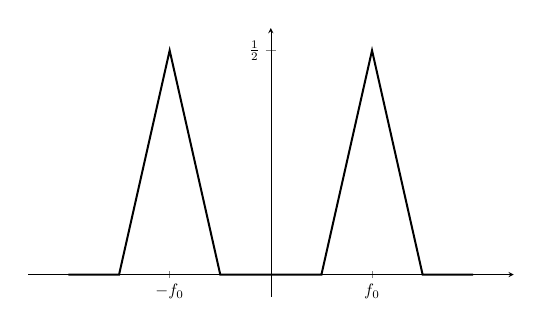
\begin{tikzpicture}[scale=.6]
	\begin{axis}[axis lines=middle,no markers,enlargelimits,xscale=1.5,xtick={-2,2},ytick={1},xticklabels={$-f_0$,$f_0$},yticklabels={$\frac{1}{2}$}]
	\addplot [very thick]coordinates {(-4,0)(-3,0)(-2,1)(-1,0)(1,0)(2,1)(3,0)(4,0)};
	\end{axis}\end{tikzpicture}
}
\caption{Esempio modulazione}
\end{figure}

\subsection{Trasformata segnali periodici}
Un segnale periodico $s(t)$ è la somma di infinite repliche di un segnale ristretto $s_T(t)$ ad un periodo $\left[-\frac{T}{2},\frac{T}{2}\right]$ e per la definizione di serie di Fourier somma di esponenziali complessi pesati da coefficienti
\begin{equation}
s(t)=\sum_{n=-\infty}^{+\infty}{s_T(t-n T)}=\sum_{k=-\infty}^{+\infty}{c_k\e{\imath 2\pi\frac{k}{T}t}}
\end{equation}

Definita la trasformata di Fourier del segnale ristretto $S_T(f)=\fourier{s_T(t)}$ si ha che i coefficienti 	\[c_k=\frac{1}{T}\intd{-\frac{T}{2}}{\frac{T}{2}}{s(t)\e{-\imath 2\pi\frac{k}{T}t}}{t}=\frac{1}{T}\intinf{s_T(t)\e{-\imath 2\pi\frac{k}{T}t}}{t}=\frac{1}{T}\f{S_T}{\frac{k}{T}}\]
quindi
\[s(t)=\frac{1}{T}\sum_{k=-\infty}^{+\infty}{\f{S_T}{\frac{k}{T}}\e{\imath 2\pi\frac{k}{T}t}}\]
\begin{equation}
S(f)=\frac{1}{T}\sum_{k=-\infty}^{+\infty}{\f{S_T}{\frac{k}{T}}\f{\delta}{f-\frac{k}{T}}}
\end{equation}
La trasformata di Fourier di un segnale periodico è la somma di infiniti impulsi a frequenza multipla della fondamentale.

\clearpage
\section{Esempi ed esercizi}
\begin{esempio}
La trasformata di un treno di impulsi è un treno di impulsi in frequenza
\[s(t)=\sum_{n=-\infty}^{+\infty}{\delta(t-n T)} \qquad S(f)=\frac{1}{T}\sum_{k=-\infty}^{+\infty}{\f{\delta}{f-\frac{k}{T}}}\]
\begin{nota}
Esempio importante per digitalizzazione e campionamento (par.\ref{sec:campionamento}).
\end{nota}

\begin{figure}[h!]
\centering
\subfloat[][$s(t)$]{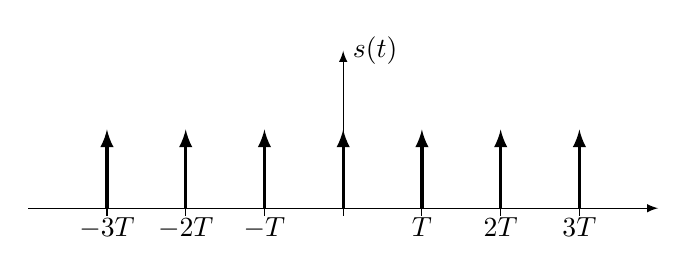
\begin{tikzpicture}
	\draw [-latex] (-4,0)--(4,0);
	\draw [-latex] (0,0)--(0,2);
	\foreach \i in {-3,...,3}
		\draw [very thick,-latex] (\i,0)--(\i,1);
	\foreach \i in {-3,...,3}
		\draw (\i,0)--(\i,-1mm);
	\node at(-3,0) [below] {$-3T$};
	\node at(-2,0) [below] {$-2T$};
	\node at(-1,0) [below] {$-T$};
	\node at(1,0) [below] {$T$};
	\node at(2,0) [below] {$2T$};
	\node at(3,0) [below] {$3T$};
	\node [right] at (0,2) {$s(t)$};
	\end{tikzpicture}
}\qquad\subfloat[][$S(f)$]{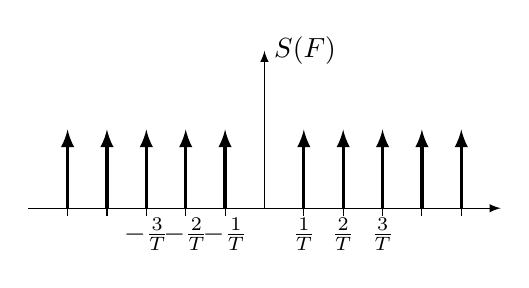
\begin{tikzpicture}
\draw [-latex] (-3,0)--(3,0);
\draw [-latex] (0,0)--(0,2);
\foreach \i in {-5,...,-1} \draw [very thick,-latex] (\i/2,0)--(\i/2,1);
\foreach \i in {1,...,5} \draw [very thick,-latex] (\i/2,0)--(\i/2,1);
\foreach \i in {-5,...,-1} \draw (\i/2,0)--(\i/2,-1mm);
\foreach \i in {1,...,5} \draw (\i/2,0)--(\i/2,-1mm);
\node at(-1.5,0) [below] {$-\frac{3}{T}$};
\node at(-1,0) [below] {$-\frac{2}{T}$};
\node at(-.5,0) [below] {$-\frac{1}{T}$};
\node at(.5,0) [below] {$\frac{1}{T}$};
\node at(1,0) [below] {$\frac{2}{T}$};
\node at(1.5,0) [below] {$\frac{3}{T}$};
\node [right] at (0,2) {$S(F)$};
\end{tikzpicture}}
\caption{Treno di impulsi nel tempo e in frequenza}
\end{figure}
\end{esempio}

\begin{esercizio}
Determinare la serie di Fourier del segnale onda triangolare in figura
\begin{figure}[h!]
\begin{center}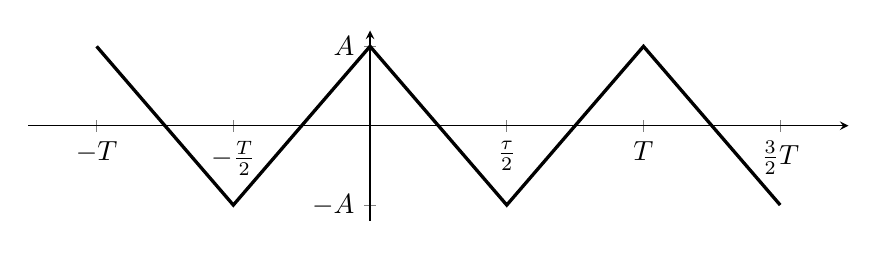
\begin{tikzpicture}
\begin{axis}[width=12cm, height=4cm, axis lines=middle,no markers,enlargelimits,xtick={-2,-1,0,1,2,3},xticklabels={$-T$,$-\frac{T}{2}$,$0$,$\frac{\tau}{2}$,$T$,$\frac{3}{2}T$},ytick={-1,0,1},yticklabels={$-A$,0,$A$}]
\addplot [very thick,domain=-2:2]coordinates {(-2,1)(-1,-1)(0,1)(1,-1)(2,1)(3,-1)};
\end{axis}
\end{tikzpicture}
\end{center}
\caption{Onda triangolare}\label{fig:onda_triangolare}
\end{figure}

\[s(t)=\sum_{k=-\infty}^{+\infty}{c_k \e{\imath 2\pi\frac{k}{T}t}} =c_0+\sum_{k=1}^{+\infty}{a_k\sen{2\pi\frac{k}{T}t}+b_k\cos{2\pi\frac{k}{T}t}}\]

Il segnale ha media nulla $c_0=0$. Il segnale è pari $a_k=0$.
\[\begin{split}b_k&=\frac{2}{T}\intd{-\frac{T}{2}}{\frac{T}{2}}{s(t)\cos{2\pi\frac{k}{T}t}}{t}=\frac{4}{T}\intd{0}{\frac{T}{2}}{s(t)\cos{2\pi\frac{k}{T}t}}{t}=\\
&=\frac{4}{T}\intd{0}{\frac{T}{2}}{\left(A-\frac{2 A}{T/2}\right)\cos{2\pi\frac{k}{T}t}}{t}=\\
&=\frac{4A}{T}\bound{0}{\frac{T}{2}}{\frac{\sen{2\pi\frac{k}{T}t}}{2\pi\frac{k}{T}}} -\frac{16A}{T^2}\intd{0}{\frac{T}{2}}{t\cos{2\pi\frac{k}{T}t}}{t}=\\
\intertext{per parti $\int u\diff v= u v-\int v\diff u$ con $u=t$, $\diff u=\diff t$, $\diff v=\cos{2\pi\frac{k}{T}t}\diff t$, $v=\frac{\sen{2\pi\frac{k}{T}t}}{2\pi\frac{k}{T}}$}
&=2A \frac{\sen{\pi k}}{\pi k}-\frac{16A}{T^2}{\left\lbrace \bound{0}{\frac{T}{2}}{t\frac{\sen{2\pi\frac{k}{T}t}}{2\pi\frac{k}{T}}}-\intd{0}{\frac{T}{2}}{\frac{\sen{2\pi\frac{k}{T}t}}{2\pi\frac{k}{T}}}{t}\right\rbrace}=\\
&=2A \frac{\sen{\pi k}}{\pi k}-\frac{16A}{T^2}{\left\lbrace\frac{T}{2}\frac{\sen{\pi k}}{2\pi\frac{k}{T}}-\bound{0}{\frac{T}{2}}{\frac{\cos{2\pi\frac{k}{T}t}}{\left(2\pi\frac{k}{T}\right)^2}}\right\rbrace}=\\
&=2A \frac{\sen{\pi k}}{\pi k}-\frac{16A}{T^2}{\left\lbrace\frac{T^2}{4}\frac{\sen{\pi k}}{\pi k}-\frac{\cos{\pi k}}{\left(2\pi\frac{k}{T}\right)^2}-\frac{1}{\left(2\pi\frac{k}{T}\right)^2}\right\rbrace}=\\
&=2A \frac{\sen{\pi k}}{\pi k}-4A{\left\lbrace\frac{\sen{\pi k}}{\pi k}-\frac{\cos{\pi k}}{\left(\pi k\right)^2}-\frac{1}{\left(\pi k\right)^2}\right\rbrace}=\\
\intertext{dove $\sen{\pi k}=0$ per $k=1,\dots+\infty$, $\cos{\pi k}=+1$ per k dispari, $-1$ per k pari}
&=\frac{4A}{(\pi k)^2}\left[1-\cos{\pi k}\right] = \frac{4A}{(\pi k)^2}\left[1-(-1)^k\right]
\end{split}\]
\end{esercizio}

\begin{esercizio}Calcolare energia e intensità spettrale di energia del segnale
\[x(t)=A\rect{\frac{t}{2T}}\]
Il segnale ha trasformata $\quad X(f)=A 2 T \sinc{2 f T}$\\
Il segnale ha energia
\[E_x=\intinf{\abs{x(t)}^2}{t}=2 A^2 T\]
Il segnale ha spettro di energia
\[\abs{X(f)}^2=(2 A T)^2\Sinc^2{2 f T}\]
\end{esercizio}
\begin{esercizio}
Calcolare energia e intensità spettrale di energia del segnale
\[y(t)=D\e{-\alpha t}\step(t)\]
Il segnale ha trasformata
\[\begin{split}Y(f)&=\intinf{ D\e{-\alpha t}\e{-\imath 2\pi f t}}{t}=D\intd{0}{+\infty}{\e{-(\alpha+\imath 2\pi f)t}}{t}=\\
&=\bound{0}{+\infty}{-\frac{D}{\alpha+\imath 2\pi f}\e{-(\alpha+\imath 2\pi f)t}}=\frac{D}{\alpha+\imath 2\pi f}\end{split}\]
Il segnale ha energia
\[E_y=\intinf{\abs{y(t)}^2}{t}=\intd{0}{+\infty}{D^2\e{-2\alpha t}}{t}=\bound{0}{+\infty}{\frac{D^2}{-2\alpha}\e{-2\alpha}}=\frac{D^2}{2\alpha}\]
Il segnale ha spettro di energia
\[\abs{Y(f)}=\frac{D^2}{\abs{\alpha+\imath 2\pi f}^2}=\frac{D^2}{\alpha^2+(2\pi f)^2}\]
\end{esercizio}
\begin{esercizio}
Calcolare la trasformata di Fourier del segnale
\[x(t)=\f{\Cos^2}{2\pi\frac{t}{T_0}}\]

ricordando che $\Cos^2 x=\frac{1}{2}+\frac{1}{2}\cos{2x}$ si ottiene
\[x(t)=\frac{1}{2}+\frac{1}{2}\cos{4\pi\frac{t}{T_0}}\]
\[X(f)=\frac{1}{2}\delta(f)+\frac{\f{\delta}{f-\frac{2}{T_0}}+\f{\delta}{f+\frac{2}{T_0}}}{4}\]
Si hanno tre righe spettrali: la componente continua, è assente la prima armonica $\frac{1}{T_0}$, si hanno due righe a frequenza doppia della fondamentale.
\begin{figure}[h!]
\centering\begin{tikzpicture}
\draw [-latex] (-3,0)--(3,0);
\draw [-latex] (0,0)--(0,2.5);
\draw [very thick,-latex] (-2,0)--(-2,1);
\draw [very thick,-latex] (0,0)--(0,2);
\draw [very thick,-latex] (2,0)--(2,1);
\draw (-2,0) -- (-2,-1mm) node [below] {$-\frac{2}{T_0}$};
\draw (-1,0) -- (-1,-1mm) node [below] {$-\frac{1}{T_0}$};
\draw (0,0) -- (0,-1mm) node [below] {$0$};
\draw (1,0) -- (1,-1mm) node [below] {$\frac{1}{T_0}$};
\draw (2,0) -- (2,-1mm) node [below] {$\frac{2}{T_0}$};
\node [right] at (0,2.5) {$X(f)$};
\end{tikzpicture}
\end{figure}
\end{esercizio}
